% \documentclass{beamer}

% \usepackage[brazil]{babel}
% \usepackage[utf8x]{inputenc}

% \title{Método Automático de Contagem Volumétrica de Veículos baseado em Visão Computacional}
% \author{Arthur Ferreira Bailão}

% \begin{document}
%   \frame{\titlepage}

%   \section{Sumário}
%   \frame{\tableofcontents}
  
% \end{document}

% $Header: /Users/joseph/Documents/LaTeX/beamer/solutions/conference-talks/conference-ornate-20min.en.tex,v 90e850259b8b 2007/01/28 20:48:30 tantau $

\documentclass{beamer}

% This file is a solution template for:

% - Talk at a conference/colloquium.
% - Talk length is about 20min.
% - Style is ornate.



% Copyright 2004 by Till Tantau <tantau@users.sourceforge.net>.
%
% In principle, this file can be redistributed and/or modified under
% the terms of the GNU Public License, version 2.
%
% However, this file is supposed to be a template to be modified
% for your own needs. For this reason, if you use this file as a
% template and not specifically distribute it as part of a another
% package/program, I grant the extra permission to freely copy and
% modify this file as you see fit and even to delete this copyright
% notice. 


\mode<presentation>
{
  \usetheme{Warsaw}
  % or ...

  \setbeamercovered{transparent}
  % or whatever (possibly just delete it)
}


\usepackage[brazil]{babel}
% or whatever

\usepackage[utf8x]{inputenc}
% or whatever
\usepackage{dcolumn}
\usepackage{times}
% \usepackage[T1]{fontenc}

% Or whatever. Note that the encoding and the font should match. If T1
% does not look nice, try deleting the line with the fontenc.


\title[Contagem Volumétrica e Visão Computacional] % (optional, use only with long paper titles)
{Método Automático de Contagem Volumétrica de Veículos baseado em Visão Computacional}

% \subtitle
% {Include Only If Paper Has a Subtitle}

\author[Arthur Bailão] % (optional, use only with lots of authors)
{Arthur Ferreira Bailão{\texorpdfstring{\\\footnotesize Orientador: Prof. Hermes Aguiar Magalhães\\Supervisora: Profª. Leise Kelli de Oliveira}{\footnotesize Orientador: Prof. Hermes Aguiar Magalhães Supervisora: Profª. Leise Kelli de Oliveira}}}
% - Give the names in the same order as the appear in the paper.
% - Use the \inst{?} command only if the authors have different
%   affiliation.

\institute % (optional, but mostly needed)
{Universidade Federal de Minas Gerais}
% - Use the \inst command only if there are several affiliations.
% - Keep it simple, no one is interested in your street address.

\date % (optional, should be abbreviation of conference name)
{Projeto Final de Curso}
% - Either use conference name or its abbreviation.
% - Not really informative to the audience, more for people (including
%   yourself) who are reading the slides online

% \subject{Theoretical Computer Science}
% This is only inserted into the PDF information catalog. Can be left
% out. 



% If you have a file called "university-logo-filename.xxx", where xxx
% is a graphic format that can be processed by latex or pdflatex,
% resp., then you can add a logo as follows:

\pgfdeclareimage[height=0.5cm]{university-logo}{imgs/principal_ufmg}
\logo{\pgfuseimage{university-logo}}



% Delete this, if you do not want the table of contents to pop up at
% the beginning of each subsection:
\AtBeginSubsection[]
{
  \begin{frame}<beamer>{Sumário}
    \tableofcontents[currentsection,currentsubsection]
  \end{frame}
}


% If you wish to uncover everything in a step-wise fashion, uncomment
% the following command: 

%\beamerdefaultoverlayspecification{<+->}


\begin{document}

\begin{frame}
  \titlepage
\end{frame}

\begin{frame}{Sumário}
  \tableofcontents
  % You might wish to add the option [pausesections]
\end{frame}


% Structuring a talk is a difficult task and the following structure
% may not be suitable. Here are some rules that apply for this
% solution: 

% - Exactly two or three sections (other than the summary).
% - At *most* three subsections per section.
% - Talk about 30s to 2min per frame. So there should be between about
%   15 and 30 frames, all told.

% - A conference audience is likely to know very little of what you
%   are going to talk about. So *simplify*!
% - In a 20min talk, getting the main ideas across is hard
%   enough. Leave out details, even if it means being less precise than
%   you think necessary.
% - If you omit details that are vital to the proof/implementation,
%   just say so once. Everybody will be happy with that.

\section{Introdução} % (fold)
\label{sec:introdu_o}


% section introdu_o (end)

\section{Objetivos} % (fold)
\label{sec:objetivos}

\begin{frame}{Qual o objetivo?}
  Desenvolver um método de contagem volumétrica que auxilie na análise das condições do tráfego urbano.
  \pause

  \begin{itemize}
    \item Contagem volumétrica utilizando um método não-invasivo de \alert{SIMPLES} implementação.
    \item Utilizar imagens coletadas por uma câmera digital.
    \item Determinar a qualidade do método.
    \item Identificar pontos de acerto e erro que podem ser trabalhados.
  \end{itemize}
\end{frame}

% section objetivos (end)

\section{Metodologia} % (fold)
\label{sec:metodologia}

\subsection{Características de captura} % (fold)
\label{sub:caracter_sticas_de_captura}

% subsection caracter_sticas_de_captura (end)

\subsection{Fluxo de processos} % (fold)
\label{sub:fluxo_de_processos}

\begin{frame}{Fluxograma global do método de contagem}
  \begin{center}
    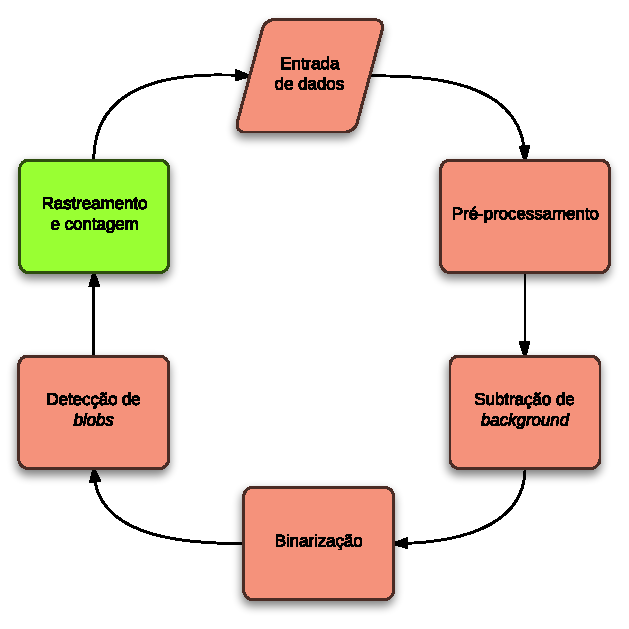
\includegraphics[scale=0.55]{imgs/general_process.pdf}
  \end{center}
\end{frame}

\begin{frame}{Entrada de dados}
  \begin{columns}[T]
    \begin{column}{.5\textwidth}
      \begin{itemize}
        \item Imagens capturadas previamente.
        \item Os \textit{frames} são obtidos individualmente.
        \item Abstração de um arquivo de vídeo por uma sequência de imagens.
      \end{itemize}
    \end{column}
    \begin{column}{.5\textwidth}
      \begin{block}{}
        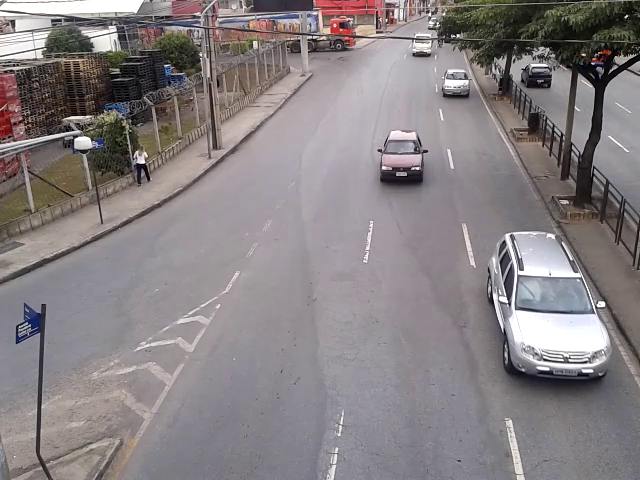
\includegraphics[width=\textwidth]{imgs/frame.png}
      \end{block}
    \end{column}
  \end{columns}
\end{frame}

\begin{frame}{Pré-processamento}
  \begin{columns}[T]
    \begin{column}{.5\textwidth}
      \begin{itemize}
        \item<1-> Conversão da imagem de entrada para \textit{grayscale}.
        \item<2-> Filtragem linear gaussiana.
      \end{itemize}
    \end{column}
    \begin{column}{.5\textwidth}
      \begin{block}{}
        \includegraphics<1>[width=\textwidth]{imgs/frame_gray.png}
        \includegraphics<2>[width=\textwidth]{imgs/gray.png}
      \end{block}
    \end{column}
  \end{columns}
\end{frame}

\begin{frame}{Subtração de \textit{background}}
  \begin{columns}[T]
    \begin{column}{.5\textwidth}
      \begin{itemize}
        \item Operação complexa e de alto custo computacional, mas de simples utilização.
        \item Modelo adaptativo de mistura de gaussianas com detecção de sombras, baseado em Zivkovic[2004] e Zivkovic \& van der Heijden [2006].
      \end{itemize}
    \end{column}
    \begin{column}{.5\textwidth}
      \begin{block}{}
        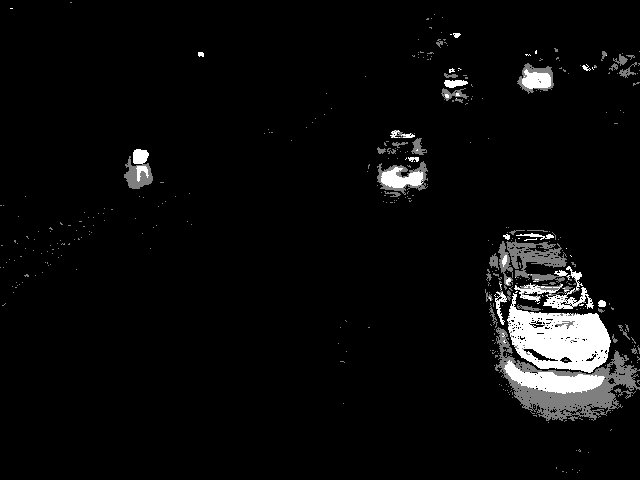
\includegraphics[width=\textwidth]{imgs/foreground.png}
      \end{block}
    \end{column}
  \end{columns}
\end{frame}

\begin{frame}{Binarização}
  \begin{columns}[T]
    \begin{column}{.5\textwidth}
      \begin{itemize}
        \item<1-> Segmentar as regiões de interesse.
        \item<1-> Operação de limiarização ou \textit{thresholding}.
        \item<2-> Operação morfológica de fechamento.
        \item<2-> Uniformizar a região de segmentação dos objetos.
      \end{itemize}
    \end{column}
    \begin{column}{.5\textwidth}
      \begin{block}{}
        \includegraphics<1>[width=\textwidth]{imgs/bin.png}
        \includegraphics<2>[width=\textwidth]{imgs/morph.png}
      \end{block}
    \end{column}
  \end{columns}
\end{frame}

\begin{frame}{Detecção de \textit{blobs}}
  \begin{columns}[T]
    \begin{column}{.5\textwidth}
      
    \end{column}
    \begin{column}{.5\textwidth}
      \begin{block}{}
        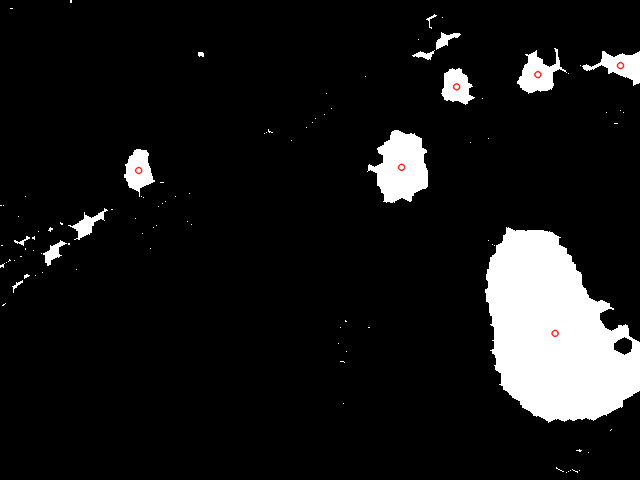
\includegraphics[width=\textwidth]{imgs/keypoints.png}
      \end{block}
    \end{column}
  \end{columns}
\end{frame}

\begin{frame}{Rastreamento e contagem}
  \begin{columns}[T]
    \begin{column}{.5\textwidth}
      
    \end{column}
    \begin{column}{.5\textwidth}
      \begin{block}{}
        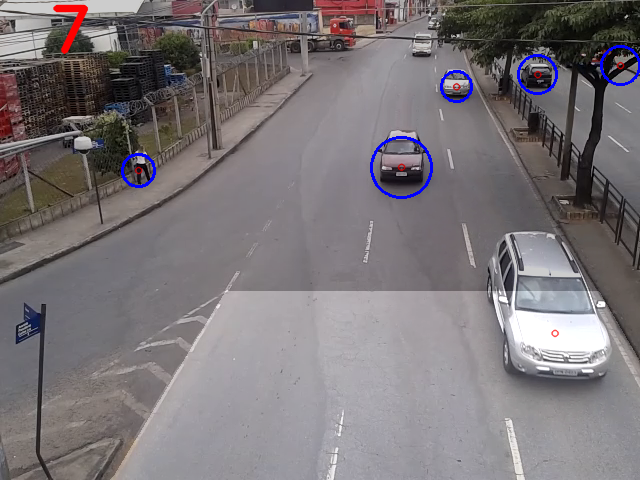
\includegraphics[width=\textwidth]{imgs/trackers.png}
      \end{block}{}
    \end{column}
  \end{columns}
\end{frame}

\begin{frame}{Rastreamento e contagem}
  \begin{center}
    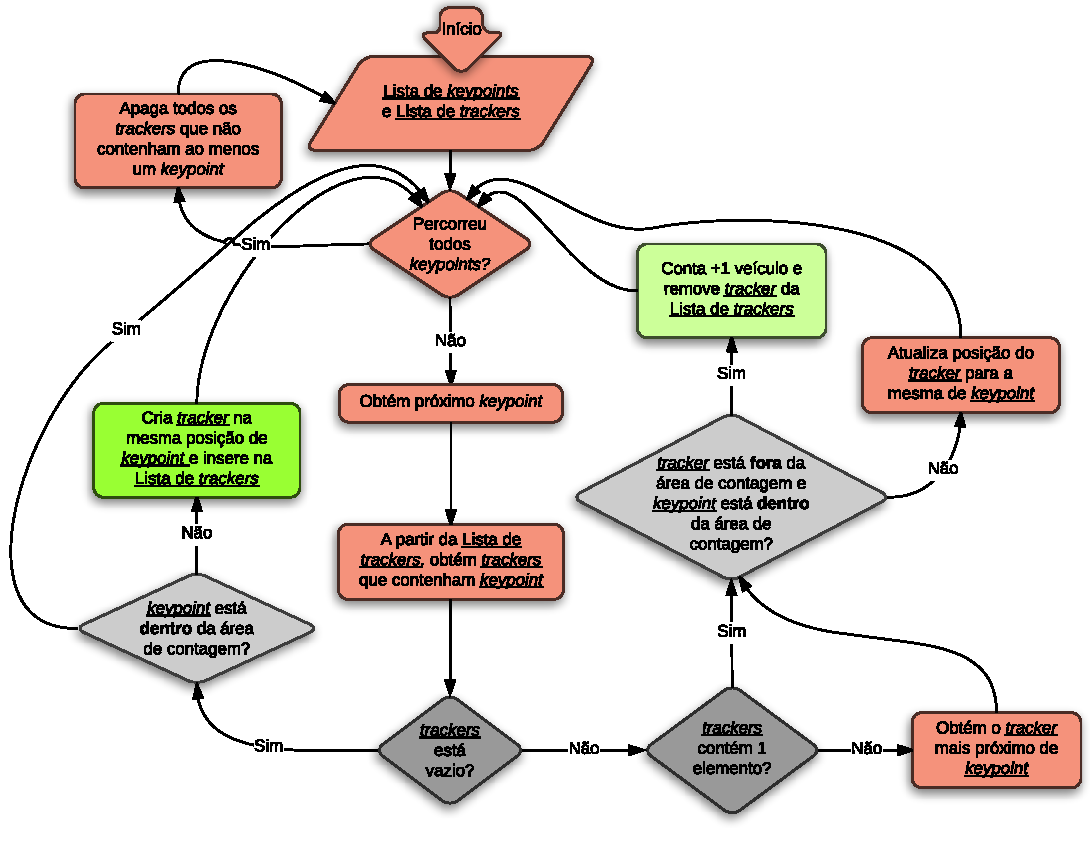
\includegraphics[scale=0.417]{imgs/fluxograma_contagem.pdf}
  \end{center}
\end{frame}

% subsection fluxo_de_processos (end)

\subsection{Avaliação dos resultados} % (fold)
\label{sub:avalia_o_dos_resultados}

\begin{frame}{A Matriz de confusão}
  
\end{frame}

\begin{frame}{Como calcular os índices de desempenho}{Precisão (P), \textit{Recall} (R) e Acurácia (A)}
  \begin{equation}
    \label{eq:precisao}
    P=\dfrac{VP}{VP+FP}
  \end{equation}

  \begin{equation}
    \label{eq:recall}
    R=\dfrac{VP}{VP+FN}
  \end{equation}

  \begin{equation}
    \label{eq:acuracia}
    A=\dfrac{VP+VN}{VP+FP+FN+VN}
  \end{equation}
\end{frame}

\begin{frame}{Como calcular o índice Kappa (K)}
  É utilizado como uma medida apropriada da exatidão por representar inteiramente a matriz de confusão.

  \begin{equation}
    \label{eq:kappa}
    K=\dfrac{\theta_{1}-\theta_{2}}{1-\theta_{2}}
  \end{equation}

  \begin{equation*}
    \label{eq:theta_1}
    \theta_{1}=\dfrac{VP+VN}{VP+FP+FN+VN}
  \end{equation*}

  \begin{equation*}
    \label{eq:theta_2}
    \theta_{2}=\dfrac{\alpha+\beta}{\gamma^{2}}
  \end{equation*}

  $\alpha=(VP+FN)*(VP+FP)$, $\beta=(VN+FN)*(VN+FP)$ e $\gamma=VP+VN+FP+FN$.

\end{frame} 

\begin{frame}{Qualidade da contagem}{Índice Kappa (K)}
  \begin{center}
    \begin{tabular}{cc}
    \hline
    \textbf{Índice Kappa (K)} & \textbf{Qualidade} \\
    \hline
      $K < 0.2$ & Ruim \\
      $0.2 \leq K < 0.4$ & Razoável \\
      $0.4 \leq K < 0.6$ & Bom \\
      $0.6 \leq K < 0.8$ & Muito bom \\
      $K \geq 0.8$ & Excelente \\
    \hline
    \end{tabular}
  \end{center}
\end{frame}

% subsection avalia_o_dos_resultados (end)

% section metodologia (end)

\section{Motivation}

\subsection{The Basic Problem That We Studied}

\begin{frame}{Make Titles Informative. Use Uppercase Letters.}{Subtitles are optional.}
  % - A title should summarize the slide in an understandable fashion
  %   for anyone how does not follow everything on the slide itself.

  \begin{itemize}
  \item
    Use \texttt{itemize} a lot.
  \item
    Use very short sentences or short phrases.
  \end{itemize}
\end{frame}

\begin{frame}{Make Titles Informative.}

  You can create overlays\dots
  \begin{itemize}
  \item using the \texttt{pause} command:
    \begin{itemize}
    \item
      First item.
      \pause
    \item    
      Second item.
    \end{itemize}
  \item
    using overlay specifications:
    \begin{itemize}
    \item<3->
      First item.
    \item<4->
      Second item.
    \end{itemize}
  \item
    using the general \texttt{uncover} command:
    \begin{itemize}
      \uncover<5->{\item
        First item.}
      \uncover<6->{\item
        Second item.}
    \end{itemize}
  \end{itemize}
\end{frame}


\subsection{Previous Work}

\begin{frame}{Make Titles Informative.}
  % \begin{tabular}{l!{\vrule}cccc}
  % Class & A & B & C & D \\\hline
  % X
  % & 1 & 2 & 3 & 4 \pause\\
  % Y
  % & 3 & 4 & 5 & 6 \pause\\
  % Z
  % & 5 & 6 & 7 & 8
  % \end{tabular}
\end{frame}

\begin{frame}{Make Titles Informative.}
\end{frame}



\section{Our Results/Contribution}

\subsection{Main Results}

\begin{frame}{Make Titles Informative.}
\end{frame}

\begin{frame}{Make Titles Informative.}
\end{frame}

\begin{frame}{Make Titles Informative.}
\end{frame}


\subsection{Basic Ideas for Proofs/Implementation}

\begin{frame}{Make Titles Informative.}
\end{frame}

\begin{frame}{Make Titles Informative.}
\end{frame}

\begin{frame}{Make Titles Informative.}
\end{frame}



% \section*{Summary}

% \begin{frame}{Summary}

%   % Keep the summary *very short*.
%   \begin{itemize}
%   \item
%     The \alert{first main message} of your talk in one or two lines.
%   \item
%     The \alert{second main message} of your talk in one or two lines.
%   \item
%     Perhaps a \alert{third message}, but not more than that.
%   \end{itemize}
  
%   % The following outlook is optional.
%   \vskip0pt plus.5fill
%   \begin{itemize}
%   \item
%     Outlook
%     \begin{itemize}
%     \item
%       Something you haven't solved.
%     \item
%       Something else you haven't solved.
%     \end{itemize}
%   \end{itemize}
% \end{frame}



% % All of the following is optional and typically not needed. 
% \appendix
% \section<presentation>*{\appendixname}
% \subsection<presentation>*{For Further Reading}

% \begin{frame}[allowframebreaks]
%   \frametitle<presentation>{For Further Reading}
    
%   \begin{thebibliography}{10}
    
%   \beamertemplatebookbibitems
%   % Start with overview books.

%   \bibitem{Author1990}
%     A.~Author.
%     \newblock {\em Handbook of Everything}.
%     \newblock Some Press, 1990.
 
    
%   \beamertemplatearticlebibitems
%   % Followed by interesting articles. Keep the list short. 

%   \bibitem{Someone2000}
%     S.~Someone.
%     \newblock On this and that.
%     \newblock {\em Journal of This and That}, 2(1):50--100,
%     2000.
%   \end{thebibliography}
% \end{frame}

\end{document}

